\chapter{Choosing Transformer Model} \label{choosing-transformer-model}

To predict the toxicity of the post content, I evaluated three transformer-based models: Detoxify (Original), Detoxify (Unbiased) from Unitary, and Perspective API. These models predict the probability of six to seven toxicity categories.

\section{Annotation} \label{annotation}

All models were evaluated on a specific subset of the dataset. The selected timeframe was the evening of the Olympic Games' opening ceremony, chosen due to the expectation of heightened online discussions and, consequently, an increased presence of toxic content. The dataset covers the period from 20:00 to 23:00 on July 26, 2024, comprising 1,179,897 posts. This context switch which may impact the model performance, but as well shows the model's robustness in a new context.

After the models completed their predictions, a sample was drawn for each model, selecting 25 posts per toxicity category with a predicted probability greater than 0.5 for that category. The selected posts were then concatenated, and duplicates were removed, resulting in a final annotation dataset of 253 posts.

The annotation process was conducted by two researchers using Label Studio. The posts were labeled according to the following categories in the table below. The annotation of hate speech remains a highly subjective task, influenced by individual annotator biases, further affecting consistency and reliability. To ensure the reliability of the annotations, inter-annotator agreement was measured using Cohen's Kappa. The results showed perfect agreement (Cohen's Kappa = 1.0) for the categories of toxic, severe toxic, threat, insult, and identity attack. Near-perfect agreement was achieved for obscene (Cohen's Kappa = 0.9907) and sexually explicit (Cohen's Kappa = 0.9735), indicating a high level of consistency between the annotators.

\begin{table}[h]
    \centering
    \renewcommand{\arraystretch}{1.3}
    \begin{tabularx}{\textwidth}{lX}
        \toprule
        \textbf{Category} & \textbf{Description} \\
        \midrule
        TOXIC & A rude, disrespectful, or unreasonable comment that is likely to make someone leave a discussion. \\
        SEVERE TOXIC & A very hateful, aggressive, or disrespectful comment that is highly likely to push someone away. \\
        IDENTITY ATTACK & Negative or hateful comments targeting someone because of their identity. \\
        INSULT & Insulting, inflammatory, or negative comments towards a person or group. \\
        OBSCENE & Swear words, curse words, or other obscene or profane language. \\
        THREAT & Describes an intention to inflict pain, injury, or violence against an individual or group. \\
        SEXUALLY EXPLICIT & Genital nudity or descriptions of simulated or actual sexual acts. \\
        \bottomrule
    \end{tabularx}
    \caption{Toxicity Categories and Their Descriptions}
\end{table}

\section{Evaluation} \label{evaluation}

In the evaluation of the toxicity detection models, the analysis focused on the probability distributions of toxicity categories across three models: the Perspective API and two Detoxify models (original and unbiased). The evaluation did not involve optimizing prediction thresholds; instead, a fixed threshold of 0.5 was used to compare the F1 scores. The results indicated that the Perspective API model generally outperformed the Detoxify models in terms of F1 score across most toxicity categories. However, a closer examination of the probability distributions revealed notable differences in the models' behavior. The Perspective API model exhibited a widely spread probability distribution, suggesting a more cautious and less confident approach to predictions. In contrast, the Detoxify models demonstrated a more concentrated probability distribution, indicating higher confidence in their predictions.

\begin{figure}[h]
    \centering
    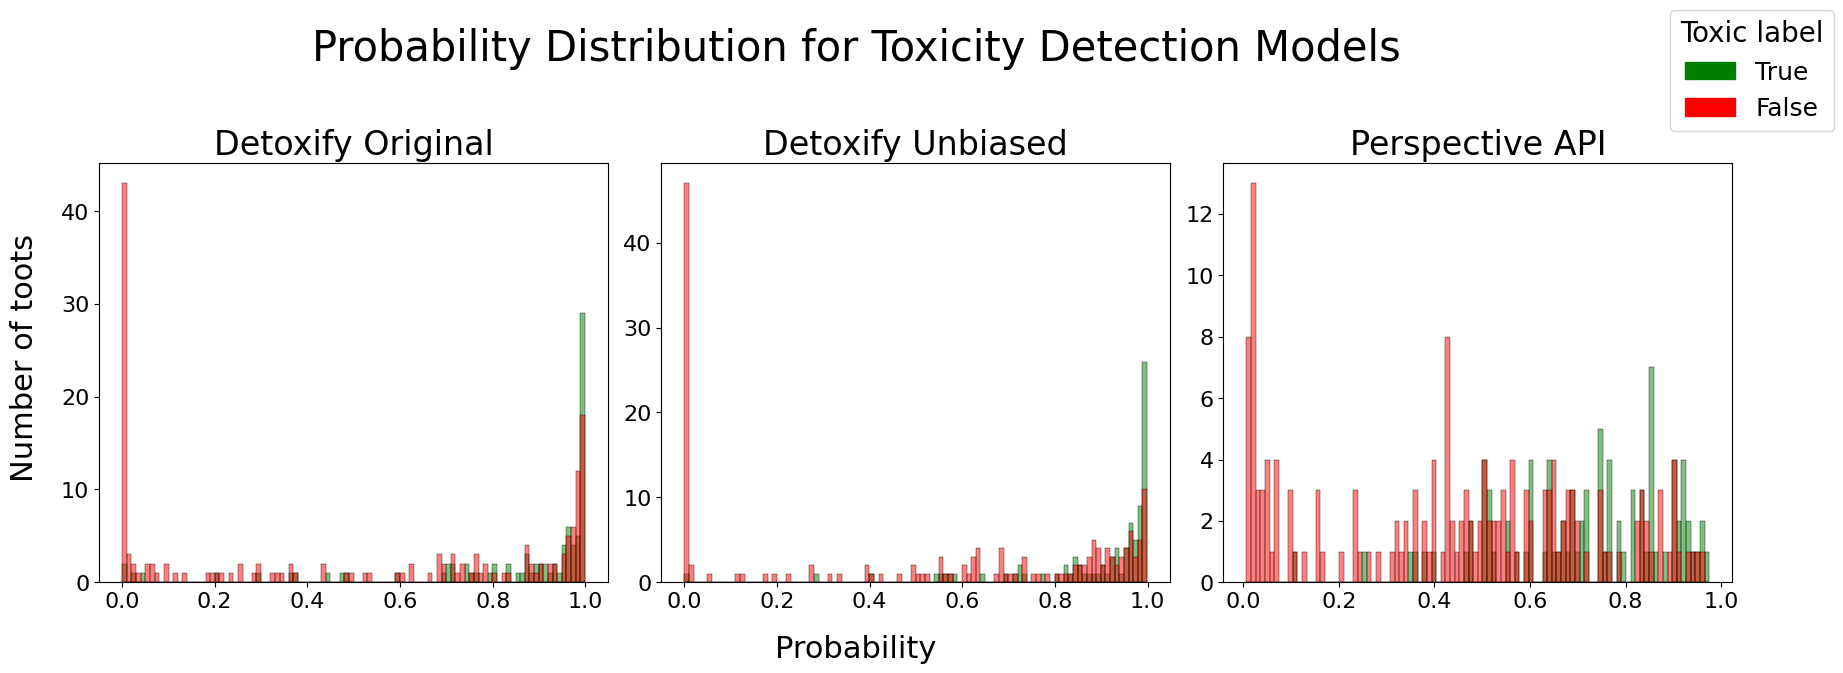
\includegraphics[width=\textwidth]{../material/probability_distribution.png}
    \caption{Probability Distribution of Toxicity category across the three models}
    \label{fig:probability-distribution}
\end{figure}

While the Perspective API model's performance metrics were stronger, its limited accessibility, restricted by a low request rate and lack of open access, posed significant practical limitations for large-scale analysis. On the other hand, the Detoxify models, being open-source, offered unrestricted usage, making them more suitable for extensive studies. Given that the primary objective of this research is not to predict toxicity in individual posts but to analyze broader trends in toxicity across Mastodon instances, the Detoxify models were considered more appropriate. A confident model, such as Detoxify, is better suited for identifying and tracking trends over time.

Between the two Detoxify models, the unbiased version was selected for further analysis due to its superior performance and the inclusion of an additional category, "sexual explicit," which is absent in the original Detoxify model. However, it is important to note that the "severe toxic" label in the Detoxify unbiased model demonstrated poor performance, likely due to the limited number of supporting posts (only 10 in the dataset). Consequently, findings related to this category should be interpreted with caution. Despite this limitation, the Detoxify unbiased model was chosen as the most suitable tool for analyzing toxicity trends in Mastodon communities, balancing performance, accessibility, and practical applicability.


\begin{table}[h!]
\centering
\begin{tabular}{|l|l|c|c|c|c|}
\hline
\textbf{Model} & \textbf{Category} & \textbf{F1} & \textbf{Precision} & \textbf{Recall} & \textbf{Support} \\
\hline
Detoxify Original & & 0.622 & 0.482 & 0.878 & 90 \\
Detoxify Unbiased & toxic & 0.635 & 0.473 & 0.967 & 90 \\
Perspective API & & \textbf{0.664} & 0.526 & 0.900 & 90 \\
\hline
Detoxify Original & & 0.148 & 0.118 & 0.200 & 10 \\
Detoxify Unbiased & severe toxic & 0.000 & 0.000 & 0.000 & 10 \\
Perspective API & & \textbf{0.222} & 0.176 & 0.300 & 10 \\
\hline
Detoxify Original & & \textbf{0.741} & 0.613 & 0.936 & 78 \\
Detoxify Unbiased & obscene & 0.739 & 0.642 & 0.872 & 78 \\
Perspective API & & 0.738 & 0.615 & 0.923 & 78 \\
\hline
Detoxify Original & & 0.462 & 0.429 & 0.500 & 18 \\
Detoxify Unbiased & threat & 0.520 & 0.406 & 0.722 & 18 \\
Perspective API & & \textbf{0.596} & 0.483 & 0.778 & 18 \\
\hline
Detoxify Original & & 0.377 & 0.312 & 0.476 & 42 \\
Detoxify Unbiased & insult & \textbf{0.500} & 0.378 & 0.738 & 42 \\
Perspective API & & 0.487 & 0.384 & 0.667 & 42 \\
\hline
Detoxify Original & & 0.440 & 0.314 & 0.733 & 15 \\
Detoxify Unbiased & identity attack & \textbf{0.545} & 0.414 & 0.800 & 15 \\
Perspective API & & 0.456 & 0.310 & 0.867 & 15 \\
\hline
Detoxify Original & & 0.000 & 0.000 & 0.000 & 21 \\
Detoxify Unbiased & sexually explicit & 0.392 & 0.333 & 0.476 & 21 \\
Perspective API & & \textbf{0.576} & 0.447 & 0.810 & 21 \\
\hline
\end{tabular}
\caption{Performance Metrics with Highlighted Highest F1 Scores}
\end{table}

\section{Detoxify Unbiased} \label{detoxify-unbiased}

The Unbiased Detoxify model is built on the RoBERTa-base architecture, which is a robust transformer model trained specifically for toxicity classification tasks. It was trained using the Jigsaw Unintended Bias in Toxicity Classification Challenge dataset, which includes labeled data for both general toxicity and toxicity directed toward specific identity groups. This makes it a critical tool in distinguishing between harmful general toxic language and toxic language targeting vulnerable identities, such as race, gender, and religion.

The model utilizes a combined loss function during training, which incorporates both toxicity and identity labels. This ensures that the model learns to minimize unintended bias, especially in cases where comments contain identity-related toxicity. A bias metric is also employed to evaluate how well the model performs across various identity subgroups, with the aim of reducing unfair bias in its predictions. \citep{detoxify:medium}